% Options for packages loaded elsewhere
\PassOptionsToPackage{unicode}{hyperref}
\PassOptionsToPackage{hyphens}{url}
%
\documentclass[
]{article}
\usepackage{amsmath,amssymb}
\usepackage{lmodern}
\usepackage{ifxetex,ifluatex}
\ifnum 0\ifxetex 1\fi\ifluatex 1\fi=0 % if pdftex
  \usepackage[T1]{fontenc}
  \usepackage[utf8]{inputenc}
  \usepackage{textcomp} % provide euro and other symbols
\else % if luatex or xetex
  \usepackage{unicode-math}
  \defaultfontfeatures{Scale=MatchLowercase}
  \defaultfontfeatures[\rmfamily]{Ligatures=TeX,Scale=1}
\fi
% Use upquote if available, for straight quotes in verbatim environments
\IfFileExists{upquote.sty}{\usepackage{upquote}}{}
\IfFileExists{microtype.sty}{% use microtype if available
  \usepackage[]{microtype}
  \UseMicrotypeSet[protrusion]{basicmath} % disable protrusion for tt fonts
}{}
\makeatletter
\@ifundefined{KOMAClassName}{% if non-KOMA class
  \IfFileExists{parskip.sty}{%
    \usepackage{parskip}
  }{% else
    \setlength{\parindent}{0pt}
    \setlength{\parskip}{6pt plus 2pt minus 1pt}}
}{% if KOMA class
  \KOMAoptions{parskip=half}}
\makeatother
\usepackage{xcolor}
\IfFileExists{xurl.sty}{\usepackage{xurl}}{} % add URL line breaks if available
\IfFileExists{bookmark.sty}{\usepackage{bookmark}}{\usepackage{hyperref}}
\hypersetup{
  pdftitle={Lab-19-Pertussis},
  pdfauthor={Ethan},
  hidelinks,
  pdfcreator={LaTeX via pandoc}}
\urlstyle{same} % disable monospaced font for URLs
\usepackage[margin=1in]{geometry}
\usepackage{color}
\usepackage{fancyvrb}
\newcommand{\VerbBar}{|}
\newcommand{\VERB}{\Verb[commandchars=\\\{\}]}
\DefineVerbatimEnvironment{Highlighting}{Verbatim}{commandchars=\\\{\}}
% Add ',fontsize=\small' for more characters per line
\usepackage{framed}
\definecolor{shadecolor}{RGB}{248,248,248}
\newenvironment{Shaded}{\begin{snugshade}}{\end{snugshade}}
\newcommand{\AlertTok}[1]{\textcolor[rgb]{0.94,0.16,0.16}{#1}}
\newcommand{\AnnotationTok}[1]{\textcolor[rgb]{0.56,0.35,0.01}{\textbf{\textit{#1}}}}
\newcommand{\AttributeTok}[1]{\textcolor[rgb]{0.77,0.63,0.00}{#1}}
\newcommand{\BaseNTok}[1]{\textcolor[rgb]{0.00,0.00,0.81}{#1}}
\newcommand{\BuiltInTok}[1]{#1}
\newcommand{\CharTok}[1]{\textcolor[rgb]{0.31,0.60,0.02}{#1}}
\newcommand{\CommentTok}[1]{\textcolor[rgb]{0.56,0.35,0.01}{\textit{#1}}}
\newcommand{\CommentVarTok}[1]{\textcolor[rgb]{0.56,0.35,0.01}{\textbf{\textit{#1}}}}
\newcommand{\ConstantTok}[1]{\textcolor[rgb]{0.00,0.00,0.00}{#1}}
\newcommand{\ControlFlowTok}[1]{\textcolor[rgb]{0.13,0.29,0.53}{\textbf{#1}}}
\newcommand{\DataTypeTok}[1]{\textcolor[rgb]{0.13,0.29,0.53}{#1}}
\newcommand{\DecValTok}[1]{\textcolor[rgb]{0.00,0.00,0.81}{#1}}
\newcommand{\DocumentationTok}[1]{\textcolor[rgb]{0.56,0.35,0.01}{\textbf{\textit{#1}}}}
\newcommand{\ErrorTok}[1]{\textcolor[rgb]{0.64,0.00,0.00}{\textbf{#1}}}
\newcommand{\ExtensionTok}[1]{#1}
\newcommand{\FloatTok}[1]{\textcolor[rgb]{0.00,0.00,0.81}{#1}}
\newcommand{\FunctionTok}[1]{\textcolor[rgb]{0.00,0.00,0.00}{#1}}
\newcommand{\ImportTok}[1]{#1}
\newcommand{\InformationTok}[1]{\textcolor[rgb]{0.56,0.35,0.01}{\textbf{\textit{#1}}}}
\newcommand{\KeywordTok}[1]{\textcolor[rgb]{0.13,0.29,0.53}{\textbf{#1}}}
\newcommand{\NormalTok}[1]{#1}
\newcommand{\OperatorTok}[1]{\textcolor[rgb]{0.81,0.36,0.00}{\textbf{#1}}}
\newcommand{\OtherTok}[1]{\textcolor[rgb]{0.56,0.35,0.01}{#1}}
\newcommand{\PreprocessorTok}[1]{\textcolor[rgb]{0.56,0.35,0.01}{\textit{#1}}}
\newcommand{\RegionMarkerTok}[1]{#1}
\newcommand{\SpecialCharTok}[1]{\textcolor[rgb]{0.00,0.00,0.00}{#1}}
\newcommand{\SpecialStringTok}[1]{\textcolor[rgb]{0.31,0.60,0.02}{#1}}
\newcommand{\StringTok}[1]{\textcolor[rgb]{0.31,0.60,0.02}{#1}}
\newcommand{\VariableTok}[1]{\textcolor[rgb]{0.00,0.00,0.00}{#1}}
\newcommand{\VerbatimStringTok}[1]{\textcolor[rgb]{0.31,0.60,0.02}{#1}}
\newcommand{\WarningTok}[1]{\textcolor[rgb]{0.56,0.35,0.01}{\textbf{\textit{#1}}}}
\usepackage{graphicx}
\makeatletter
\def\maxwidth{\ifdim\Gin@nat@width>\linewidth\linewidth\else\Gin@nat@width\fi}
\def\maxheight{\ifdim\Gin@nat@height>\textheight\textheight\else\Gin@nat@height\fi}
\makeatother
% Scale images if necessary, so that they will not overflow the page
% margins by default, and it is still possible to overwrite the defaults
% using explicit options in \includegraphics[width, height, ...]{}
\setkeys{Gin}{width=\maxwidth,height=\maxheight,keepaspectratio}
% Set default figure placement to htbp
\makeatletter
\def\fps@figure{htbp}
\makeatother
\setlength{\emergencystretch}{3em} % prevent overfull lines
\providecommand{\tightlist}{%
  \setlength{\itemsep}{0pt}\setlength{\parskip}{0pt}}
\setcounter{secnumdepth}{-\maxdimen} % remove section numbering
\ifluatex
  \usepackage{selnolig}  % disable illegal ligatures
\fi

\title{Lab-19-Pertussis}
\author{Ethan}
\date{3/14/2023}

\begin{document}
\maketitle

install.packages(``datapasta'')

\hypertarget{investigating-pertussis-cases-by-year}{%
\section{Investigating pertussis cases by
year}\label{investigating-pertussis-cases-by-year}}

CDC tracking cases of Pertussis in the US. We can get their data via web
scrapping

\begin{Shaded}
\begin{Highlighting}[]
\CommentTok{\# Call ggplot2 pkg}
\FunctionTok{library}\NormalTok{(ggplot2)}
\end{Highlighting}
\end{Shaded}

Q1. With the help of the R ``addin'' package datapasta assign the CDC
pertussis case number data to a data frame called cdc and use ggplot to
make a plot of cases numbers over time.

\begin{Shaded}
\begin{Highlighting}[]
\NormalTok{cdc.plot }\OtherTok{\textless{}{-}} \FunctionTok{ggplot}\NormalTok{(cdc) }\SpecialCharTok{+}
  \FunctionTok{aes}\NormalTok{(Year, Cases) }\SpecialCharTok{+}
  \FunctionTok{geom\_point}\NormalTok{() }\SpecialCharTok{+}
  \FunctionTok{geom\_line}\NormalTok{() }\SpecialCharTok{+}
  \FunctionTok{labs}\NormalTok{(}\AttributeTok{title =} \StringTok{"Cases of Pertussis in US from 1920 to 2019"}\NormalTok{,}
       \AttributeTok{subtitle =} \StringTok{"Data from the CDC"}\NormalTok{)}
\NormalTok{cdc.plot}
\end{Highlighting}
\end{Shaded}

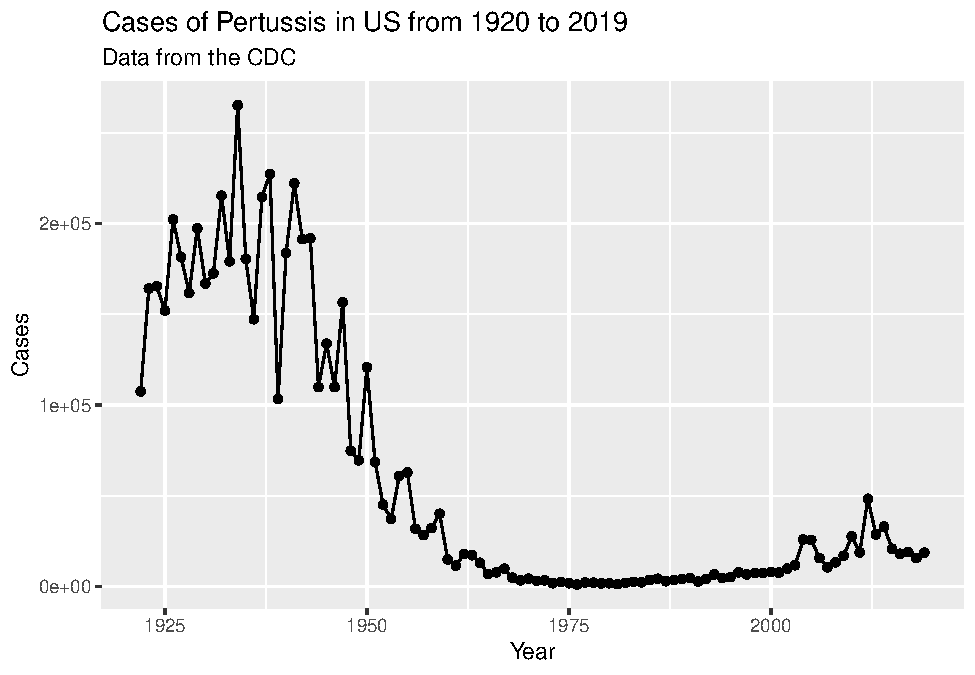
\includegraphics{lab-19-143_files/figure-latex/unnamed-chunk-3-1.pdf}

Q2. Using the ggplot geom\_vline() function add lines to your previous
plot for the 1946 introduction of the wP vaccine and the 1996 switch to
aP vaccine (see example in the hint below). What do you notice?

\begin{Shaded}
\begin{Highlighting}[]
\NormalTok{cdc.plot }\SpecialCharTok{+} 
  \FunctionTok{geom\_vline}\NormalTok{(}\AttributeTok{xintercept =} \DecValTok{1946}\NormalTok{, }\AttributeTok{linetype =} \DecValTok{2}\NormalTok{ ,}\AttributeTok{color =} \StringTok{"blue"}\NormalTok{) }\SpecialCharTok{+}
  \FunctionTok{geom\_vline}\NormalTok{(}\AttributeTok{xintercept =} \DecValTok{1996}\NormalTok{, }\AttributeTok{linetype =} \DecValTok{2}\NormalTok{ ,}\AttributeTok{color =} \StringTok{"red"}\NormalTok{)}
\end{Highlighting}
\end{Shaded}

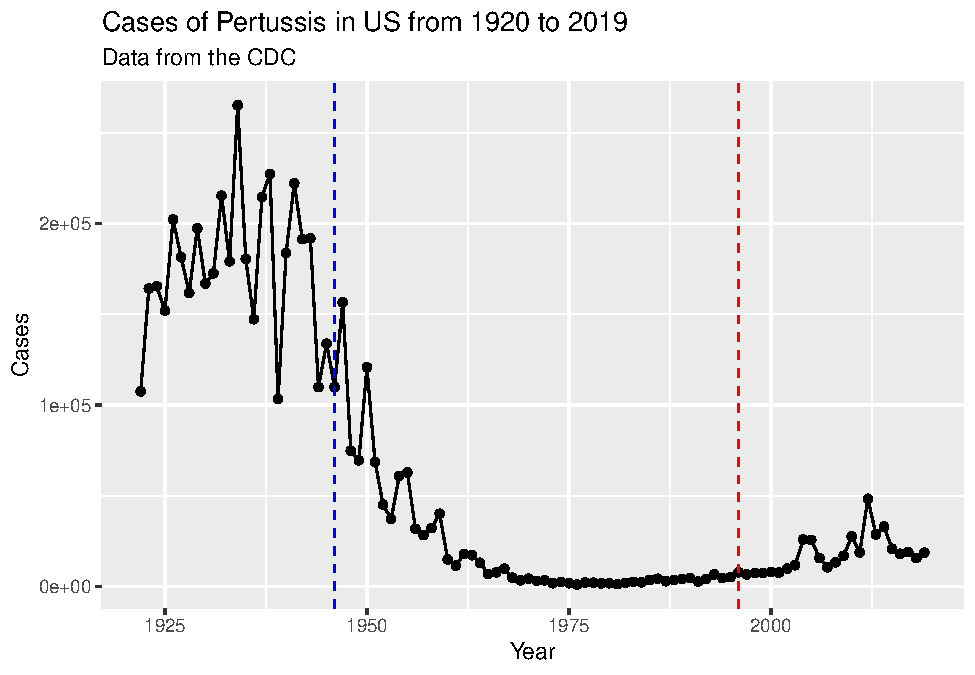
\includegraphics{lab-19-143_files/figure-latex/unnamed-chunk-4-1.pdf}

Q3. Describe what happened after the introduction of the aP vaccine? Do
you have a possible explanation for the observed trend?

The introduction of the aP vaccine in 1996 showed a continued ``low'' of
cases of pertussis from the wP vaccine. But, the cases started to
increase afterwards. Maybe, the aP vaccine just isn't as effective.

\hypertarget{cmi-pb-project}{%
\section{CMI-PB Project}\label{cmi-pb-project}}

Collest data on aP\_ and wP individuals and their immune response to
infection/booster shots

CMI-PB returns in JSON format.

On Console: install.packages(``jsonlite'')

\begin{Shaded}
\begin{Highlighting}[]
\CommentTok{\# Allows us to read, write and process JSON data}
\FunctionTok{library}\NormalTok{(jsonlite)}
\end{Highlighting}
\end{Shaded}

\begin{Shaded}
\begin{Highlighting}[]
\CommentTok{\# Read in data}
\NormalTok{subject }\OtherTok{\textless{}{-}} \FunctionTok{read\_json}\NormalTok{(}\StringTok{"https://www.cmi{-}pb.org/api/subject"}\NormalTok{, }\AttributeTok{simplifyVector =} \ConstantTok{TRUE}\NormalTok{) }
\FunctionTok{head}\NormalTok{(subject)}
\end{Highlighting}
\end{Shaded}

\begin{verbatim}
##   subject_id infancy_vac biological_sex              ethnicity  race
## 1          1          wP         Female Not Hispanic or Latino White
## 2          2          wP         Female Not Hispanic or Latino White
## 3          3          wP         Female                Unknown White
## 4          4          wP           Male Not Hispanic or Latino Asian
## 5          5          wP           Male Not Hispanic or Latino Asian
## 6          6          wP         Female Not Hispanic or Latino White
##   year_of_birth date_of_boost      dataset
## 1    1986-01-01    2016-09-12 2020_dataset
## 2    1968-01-01    2019-01-28 2020_dataset
## 3    1983-01-01    2016-10-10 2020_dataset
## 4    1988-01-01    2016-08-29 2020_dataset
## 5    1991-01-01    2016-08-29 2020_dataset
## 6    1988-01-01    2016-10-10 2020_dataset
\end{verbatim}

Q4. How may aP and wP infancy vaccinated subjects are in the dataset? 47
aP and 49 wP

\begin{Shaded}
\begin{Highlighting}[]
\CommentTok{\# Use table to separate the column into categories}
\FunctionTok{table}\NormalTok{(subject}\SpecialCharTok{$}\NormalTok{infancy\_vac)}
\end{Highlighting}
\end{Shaded}

\begin{verbatim}
## 
## aP wP 
## 47 49
\end{verbatim}

Q5. How many Male and Female subjects/patients are in the dataset? 66
Female and 30 Male

\begin{Shaded}
\begin{Highlighting}[]
\CommentTok{\# same logic different parameters}
\FunctionTok{table}\NormalTok{(subject}\SpecialCharTok{$}\NormalTok{biological\_sex)}
\end{Highlighting}
\end{Shaded}

\begin{verbatim}
## 
## Female   Male 
##     66     30
\end{verbatim}

Q6. What is the breakdown of race and biological sex (e.g.~number of
Asian females, White males etc\ldots)?

\begin{Shaded}
\begin{Highlighting}[]
\CommentTok{\# again, but with 2 parameters}
\FunctionTok{table}\NormalTok{(subject}\SpecialCharTok{$}\NormalTok{race, subject}\SpecialCharTok{$}\NormalTok{biological\_sex)}
\end{Highlighting}
\end{Shaded}

\begin{verbatim}
##                                            
##                                             Female Male
##   American Indian/Alaska Native                  0    1
##   Asian                                         18    9
##   Black or African American                      2    0
##   More Than One Race                             8    2
##   Native Hawaiian or Other Pacific Islander      1    1
##   Unknown or Not Reported                       10    4
##   White                                         27   13
\end{verbatim}

\begin{Shaded}
\begin{Highlighting}[]
\CommentTok{\# working with dates}
\FunctionTok{library}\NormalTok{(lubridate)}
\end{Highlighting}
\end{Shaded}

\begin{verbatim}
## 
## Attaching package: 'lubridate'
\end{verbatim}

\begin{verbatim}
## The following objects are masked from 'package:base':
## 
##     date, intersect, setdiff, union
\end{verbatim}

Q7. Using this approach determine (i) the average age of wP individuals,
(ii) the average age of aP individuals; and (iii) are they significantly
different? i) 36.36 years ii) 25.52 years

Get age in years for all subjects:

\begin{Shaded}
\begin{Highlighting}[]
\NormalTok{age\_days }\OtherTok{\textless{}{-}} \FunctionTok{today}\NormalTok{() }\SpecialCharTok{{-}} \FunctionTok{ymd}\NormalTok{(subject}\SpecialCharTok{$}\NormalTok{year\_of\_birth)}
\NormalTok{age\_years }\OtherTok{\textless{}{-}} \FunctionTok{time\_length}\NormalTok{(age\_days, }\StringTok{"years"}\NormalTok{)}
\NormalTok{subject}\SpecialCharTok{$}\NormalTok{age }\OtherTok{\textless{}{-}}\NormalTok{ age\_years}
\end{Highlighting}
\end{Shaded}

Average them:

\begin{Shaded}
\begin{Highlighting}[]
\FunctionTok{library}\NormalTok{(}\StringTok{"dplyr"}\NormalTok{)}
\end{Highlighting}
\end{Shaded}

\begin{verbatim}
## 
## Attaching package: 'dplyr'
\end{verbatim}

\begin{verbatim}
## The following objects are masked from 'package:stats':
## 
##     filter, lag
\end{verbatim}

\begin{verbatim}
## The following objects are masked from 'package:base':
## 
##     intersect, setdiff, setequal, union
\end{verbatim}

\begin{Shaded}
\begin{Highlighting}[]
\CommentTok{\# Using dplyr}
\CommentTok{\# Separate the categories first. Can use this for other things}
\NormalTok{ap.age }\OtherTok{\textless{}{-}} \FunctionTok{filter}\NormalTok{(subject, infancy\_vac }\SpecialCharTok{==} \StringTok{"aP"}\NormalTok{)}\SpecialCharTok{$}\NormalTok{age}
\NormalTok{wp.age }\OtherTok{\textless{}{-}} \FunctionTok{filter}\NormalTok{(subject, infancy\_vac }\SpecialCharTok{==} \StringTok{"wP"}\NormalTok{)}\SpecialCharTok{$}\NormalTok{age}

\FunctionTok{mean}\NormalTok{(ap.age)}
\end{Highlighting}
\end{Shaded}

\begin{verbatim}
## [1] 25.5156
\end{verbatim}

\begin{Shaded}
\begin{Highlighting}[]
\FunctionTok{mean}\NormalTok{(wp.age)}
\end{Highlighting}
\end{Shaded}

\begin{verbatim}
## [1] 36.36006
\end{verbatim}

T-test

\begin{Shaded}
\begin{Highlighting}[]
\FunctionTok{t.test}\NormalTok{(ap.age,wp.age)}
\end{Highlighting}
\end{Shaded}

\begin{verbatim}
## 
##  Welch Two Sample t-test
## 
## data:  ap.age and wp.age
## t = -12.092, df = 51.082, p-value < 2.2e-16
## alternative hypothesis: true difference in means is not equal to 0
## 95 percent confidence interval:
##  -12.644857  -9.044045
## sample estimates:
## mean of x mean of y 
##  25.51560  36.36006
\end{verbatim}

Q8. Determine the age of all individuals at time of boost?

\begin{Shaded}
\begin{Highlighting}[]
\NormalTok{subject}\SpecialCharTok{$}\NormalTok{age.boost }\OtherTok{\textless{}{-}} \FunctionTok{time\_length}\NormalTok{(}\FunctionTok{ymd}\NormalTok{(subject}\SpecialCharTok{$}\NormalTok{date\_of\_boost) }\SpecialCharTok{{-}} \FunctionTok{ymd}\NormalTok{(subject}\SpecialCharTok{$}\NormalTok{year\_of\_birth),}\StringTok{"years"}\NormalTok{)}
\NormalTok{subject}\SpecialCharTok{$}\NormalTok{age.boost}
\end{Highlighting}
\end{Shaded}

\begin{verbatim}
##  [1] 30.69678 51.07461 33.77413 28.65982 25.65914 28.77481 35.84942 34.14921
##  [9] 20.56400 34.56263 30.65845 34.56263 19.56194 23.61944 27.61944 29.56331
## [17] 36.69815 19.65777 22.73511 32.26557 25.90007 23.90144 25.90007 28.91992
## [25] 42.92129 47.07461 47.07461 29.07324 21.07324 21.07324 28.15058 24.15058
## [33] 24.15058 21.14990 21.14990 31.20876 26.20671 32.20808 27.20876 26.20671
## [41] 21.20739 20.26557 22.26420 19.32375 21.32238 19.32375 19.32375 22.41752
## [49] 20.41889 21.41821 19.47707 23.47707 20.47639 21.47570 19.47707 35.65777
## [57] 33.65914 31.65777 25.73580 24.70089 28.70089 33.73580 19.73443 34.73511
## [65] 19.73443 28.73648 27.73443 19.81109 26.77344 33.81246 25.77413 19.81109
## [73] 18.85010 19.81109 31.81109 22.81177 31.84942 19.84942 18.85010 18.85010
## [81] 19.90691 18.85010 20.90897 19.04449 20.04381 19.90691 19.90691 19.00616
## [89] 19.00616 20.04381 20.04381 20.07940 21.08145 20.07940 20.07940 20.07940
\end{verbatim}

Q9. With the help of a faceted boxplot (see below), do you think these
two groups are significantly different? Yes. There is no overlap

\begin{Shaded}
\begin{Highlighting}[]
\FunctionTok{ggplot}\NormalTok{(subject) }\SpecialCharTok{+}
  \FunctionTok{aes}\NormalTok{(}\FunctionTok{time\_length}\NormalTok{(age, }\StringTok{"year"}\NormalTok{),}
      \AttributeTok{fill=}\FunctionTok{as.factor}\NormalTok{(infancy\_vac)) }\SpecialCharTok{+}
  \FunctionTok{geom\_histogram}\NormalTok{(}\AttributeTok{show.legend=}\ConstantTok{FALSE}\NormalTok{) }\SpecialCharTok{+}
  \FunctionTok{facet\_wrap}\NormalTok{(}\FunctionTok{vars}\NormalTok{(infancy\_vac), }\AttributeTok{nrow=}\DecValTok{2}\NormalTok{) }
\end{Highlighting}
\end{Shaded}

\begin{verbatim}
## `stat_bin()` using `bins = 30`. Pick better value with `binwidth`.
\end{verbatim}

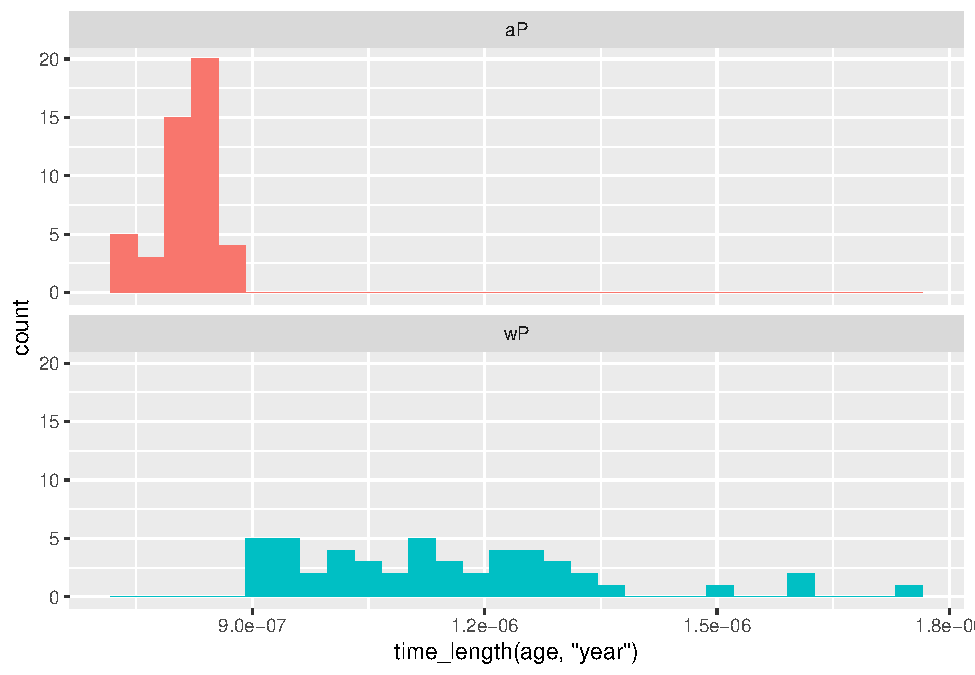
\includegraphics{lab-19-143_files/figure-latex/unnamed-chunk-16-1.pdf}

\hypertarget{joining-multiple-tables}{%
\section{Joining multiple tables}\label{joining-multiple-tables}}

\begin{Shaded}
\begin{Highlighting}[]
\CommentTok{\# New table}
\NormalTok{specimen }\OtherTok{\textless{}{-}} \FunctionTok{read\_json}\NormalTok{(}\StringTok{"http://www.cmi{-}pb.org/api/specimen"}\NormalTok{, }\AttributeTok{simplifyVector =} \ConstantTok{TRUE}\NormalTok{) }
\NormalTok{titer }\OtherTok{\textless{}{-}} \FunctionTok{read\_json}\NormalTok{(}\StringTok{"https://www.cmi{-}pb.org/api/ab\_titer"}\NormalTok{, }\AttributeTok{simplifyVector =} \ConstantTok{TRUE}\NormalTok{) }
\end{Highlighting}
\end{Shaded}

Q9. Complete the code to join specimen and subject tables to make a new
merged data frame containing all specimen records along with their
associated subject details:

\begin{Shaded}
\begin{Highlighting}[]
\FunctionTok{head}\NormalTok{(specimen)}
\end{Highlighting}
\end{Shaded}

\begin{verbatim}
##   specimen_id subject_id actual_day_relative_to_boost
## 1           1          1                           -3
## 2           2          1                          736
## 3           3          1                            1
## 4           4          1                            3
## 5           5          1                            7
## 6           6          1                           11
##   planned_day_relative_to_boost specimen_type visit
## 1                             0         Blood     1
## 2                           736         Blood    10
## 3                             1         Blood     2
## 4                             3         Blood     3
## 5                             7         Blood     4
## 6                            14         Blood     5
\end{verbatim}

\begin{Shaded}
\begin{Highlighting}[]
\FunctionTok{head}\NormalTok{(titer)}
\end{Highlighting}
\end{Shaded}

\begin{verbatim}
##   specimen_id isotype is_antigen_specific antigen        MFI MFI_normalised
## 1           1     IgE               FALSE   Total 1110.21154       2.493425
## 2           1     IgE               FALSE   Total 2708.91616       2.493425
## 3           1     IgG                TRUE      PT   68.56614       3.736992
## 4           1     IgG                TRUE     PRN  332.12718       2.602350
## 5           1     IgG                TRUE     FHA 1887.12263      34.050956
## 6           1     IgE                TRUE     ACT    0.10000       1.000000
##    unit lower_limit_of_detection
## 1 UG/ML                 2.096133
## 2 IU/ML                29.170000
## 3 IU/ML                 0.530000
## 4 IU/ML                 6.205949
## 5 IU/ML                 4.679535
## 6 IU/ML                 2.816431
\end{verbatim}

\begin{Shaded}
\begin{Highlighting}[]
\FunctionTok{dim}\NormalTok{(subject)}
\end{Highlighting}
\end{Shaded}

\begin{verbatim}
## [1] 96 10
\end{verbatim}

\begin{Shaded}
\begin{Highlighting}[]
\FunctionTok{dim}\NormalTok{(specimen)}
\end{Highlighting}
\end{Shaded}

\begin{verbatim}
## [1] 729   6
\end{verbatim}

\begin{Shaded}
\begin{Highlighting}[]
\NormalTok{meta }\OtherTok{\textless{}{-}} \FunctionTok{inner\_join}\NormalTok{(specimen, subject)}
\end{Highlighting}
\end{Shaded}

\begin{verbatim}
## Joining with `by = join_by(subject_id)`
\end{verbatim}

\begin{Shaded}
\begin{Highlighting}[]
\FunctionTok{dim}\NormalTok{(meta)}
\end{Highlighting}
\end{Shaded}

\begin{verbatim}
## [1] 729  15
\end{verbatim}

\begin{Shaded}
\begin{Highlighting}[]
\FunctionTok{head}\NormalTok{(meta)}
\end{Highlighting}
\end{Shaded}

\begin{verbatim}
##   specimen_id subject_id actual_day_relative_to_boost
## 1           1          1                           -3
## 2           2          1                          736
## 3           3          1                            1
## 4           4          1                            3
## 5           5          1                            7
## 6           6          1                           11
##   planned_day_relative_to_boost specimen_type visit infancy_vac biological_sex
## 1                             0         Blood     1          wP         Female
## 2                           736         Blood    10          wP         Female
## 3                             1         Blood     2          wP         Female
## 4                             3         Blood     3          wP         Female
## 5                             7         Blood     4          wP         Female
## 6                            14         Blood     5          wP         Female
##                ethnicity  race year_of_birth date_of_boost      dataset
## 1 Not Hispanic or Latino White    1986-01-01    2016-09-12 2020_dataset
## 2 Not Hispanic or Latino White    1986-01-01    2016-09-12 2020_dataset
## 3 Not Hispanic or Latino White    1986-01-01    2016-09-12 2020_dataset
## 4 Not Hispanic or Latino White    1986-01-01    2016-09-12 2020_dataset
## 5 Not Hispanic or Latino White    1986-01-01    2016-09-12 2020_dataset
## 6 Not Hispanic or Latino White    1986-01-01    2016-09-12 2020_dataset
##        age age.boost
## 1 37.19644  30.69678
## 2 37.19644  30.69678
## 3 37.19644  30.69678
## 4 37.19644  30.69678
## 5 37.19644  30.69678
## 6 37.19644  30.69678
\end{verbatim}

\begin{Shaded}
\begin{Highlighting}[]
\NormalTok{abdata }\OtherTok{\textless{}{-}} \FunctionTok{inner\_join}\NormalTok{(titer, meta)}
\end{Highlighting}
\end{Shaded}

\begin{verbatim}
## Joining with `by = join_by(specimen_id)`
\end{verbatim}

\begin{Shaded}
\begin{Highlighting}[]
\FunctionTok{dim}\NormalTok{(abdata)}
\end{Highlighting}
\end{Shaded}

\begin{verbatim}
## [1] 32675    22
\end{verbatim}

\begin{Shaded}
\begin{Highlighting}[]
\FunctionTok{head}\NormalTok{(abdata)}
\end{Highlighting}
\end{Shaded}

\begin{verbatim}
##   specimen_id isotype is_antigen_specific antigen        MFI MFI_normalised
## 1           1     IgE               FALSE   Total 1110.21154       2.493425
## 2           1     IgE               FALSE   Total 2708.91616       2.493425
## 3           1     IgG                TRUE      PT   68.56614       3.736992
## 4           1     IgG                TRUE     PRN  332.12718       2.602350
## 5           1     IgG                TRUE     FHA 1887.12263      34.050956
## 6           1     IgE                TRUE     ACT    0.10000       1.000000
##    unit lower_limit_of_detection subject_id actual_day_relative_to_boost
## 1 UG/ML                 2.096133          1                           -3
## 2 IU/ML                29.170000          1                           -3
## 3 IU/ML                 0.530000          1                           -3
## 4 IU/ML                 6.205949          1                           -3
## 5 IU/ML                 4.679535          1                           -3
## 6 IU/ML                 2.816431          1                           -3
##   planned_day_relative_to_boost specimen_type visit infancy_vac biological_sex
## 1                             0         Blood     1          wP         Female
## 2                             0         Blood     1          wP         Female
## 3                             0         Blood     1          wP         Female
## 4                             0         Blood     1          wP         Female
## 5                             0         Blood     1          wP         Female
## 6                             0         Blood     1          wP         Female
##                ethnicity  race year_of_birth date_of_boost      dataset
## 1 Not Hispanic or Latino White    1986-01-01    2016-09-12 2020_dataset
## 2 Not Hispanic or Latino White    1986-01-01    2016-09-12 2020_dataset
## 3 Not Hispanic or Latino White    1986-01-01    2016-09-12 2020_dataset
## 4 Not Hispanic or Latino White    1986-01-01    2016-09-12 2020_dataset
## 5 Not Hispanic or Latino White    1986-01-01    2016-09-12 2020_dataset
## 6 Not Hispanic or Latino White    1986-01-01    2016-09-12 2020_dataset
##        age age.boost
## 1 37.19644  30.69678
## 2 37.19644  30.69678
## 3 37.19644  30.69678
## 4 37.19644  30.69678
## 5 37.19644  30.69678
## 6 37.19644  30.69678
\end{verbatim}

Q11. How many specimens (i.e.~entries in abdata) do we have for each
isotype? IgE IgG IgG1 IgG2 IgG3 IgG4 6698 1413 6141 6141 6141 6141

\begin{Shaded}
\begin{Highlighting}[]
\FunctionTok{table}\NormalTok{(abdata}\SpecialCharTok{$}\NormalTok{isotype)}
\end{Highlighting}
\end{Shaded}

\begin{verbatim}
## 
##  IgE  IgG IgG1 IgG2 IgG3 IgG4 
## 6698 1413 6141 6141 6141 6141
\end{verbatim}

Q12. What do you notice about the number of visit 8 specimens compared
to other visits? 1 2 3 4 5 6 7 8 5795 4640 4640 4640 4640 4320 3920 80
It's way lower. It's still ongoing. Because the data is not complete, we
shouldn't use it.

\begin{Shaded}
\begin{Highlighting}[]
\FunctionTok{table}\NormalTok{(abdata}\SpecialCharTok{$}\NormalTok{visit)}
\end{Highlighting}
\end{Shaded}

\begin{verbatim}
## 
##    1    2    3    4    5    6    7    8 
## 5795 4640 4640 4640 4640 4320 3920   80
\end{verbatim}

Q13. Complete the following code to make a summary boxplot of Ab titer
levels for all antigens:

\begin{Shaded}
\begin{Highlighting}[]
\NormalTok{ig1 }\OtherTok{\textless{}{-}}\NormalTok{ abdata }\SpecialCharTok{\%\textgreater{}\%} \FunctionTok{filter}\NormalTok{(isotype }\SpecialCharTok{==} \StringTok{"IgG1"}\NormalTok{, visit}\SpecialCharTok{!=}\DecValTok{8}\NormalTok{)}
\FunctionTok{head}\NormalTok{(ig1)}
\end{Highlighting}
\end{Shaded}

\begin{verbatim}
##   specimen_id isotype is_antigen_specific antigen        MFI MFI_normalised
## 1           1    IgG1                TRUE     ACT 274.355068      0.6928058
## 2           1    IgG1                TRUE     LOS  10.974026      2.1645083
## 3           1    IgG1                TRUE   FELD1   1.448796      0.8080941
## 4           1    IgG1                TRUE   BETV1   0.100000      1.0000000
## 5           1    IgG1                TRUE   LOLP1   0.100000      1.0000000
## 6           1    IgG1                TRUE Measles  36.277417      1.6638332
##    unit lower_limit_of_detection subject_id actual_day_relative_to_boost
## 1 IU/ML                 3.848750          1                           -3
## 2 IU/ML                 4.357917          1                           -3
## 3 IU/ML                 2.699944          1                           -3
## 4 IU/ML                 1.734784          1                           -3
## 5 IU/ML                 2.550606          1                           -3
## 6 IU/ML                 4.438966          1                           -3
##   planned_day_relative_to_boost specimen_type visit infancy_vac biological_sex
## 1                             0         Blood     1          wP         Female
## 2                             0         Blood     1          wP         Female
## 3                             0         Blood     1          wP         Female
## 4                             0         Blood     1          wP         Female
## 5                             0         Blood     1          wP         Female
## 6                             0         Blood     1          wP         Female
##                ethnicity  race year_of_birth date_of_boost      dataset
## 1 Not Hispanic or Latino White    1986-01-01    2016-09-12 2020_dataset
## 2 Not Hispanic or Latino White    1986-01-01    2016-09-12 2020_dataset
## 3 Not Hispanic or Latino White    1986-01-01    2016-09-12 2020_dataset
## 4 Not Hispanic or Latino White    1986-01-01    2016-09-12 2020_dataset
## 5 Not Hispanic or Latino White    1986-01-01    2016-09-12 2020_dataset
## 6 Not Hispanic or Latino White    1986-01-01    2016-09-12 2020_dataset
##        age age.boost
## 1 37.19644  30.69678
## 2 37.19644  30.69678
## 3 37.19644  30.69678
## 4 37.19644  30.69678
## 5 37.19644  30.69678
## 6 37.19644  30.69678
\end{verbatim}

\begin{Shaded}
\begin{Highlighting}[]
\FunctionTok{ggplot}\NormalTok{(ig1) }\SpecialCharTok{+}
  \FunctionTok{aes}\NormalTok{(MFI,antigen) }\SpecialCharTok{+}
  \FunctionTok{geom\_boxplot}\NormalTok{() }\SpecialCharTok{+} 
  \FunctionTok{facet\_wrap}\NormalTok{(}\FunctionTok{vars}\NormalTok{(visit), }\AttributeTok{nrow=}\DecValTok{2}\NormalTok{)}
\end{Highlighting}
\end{Shaded}

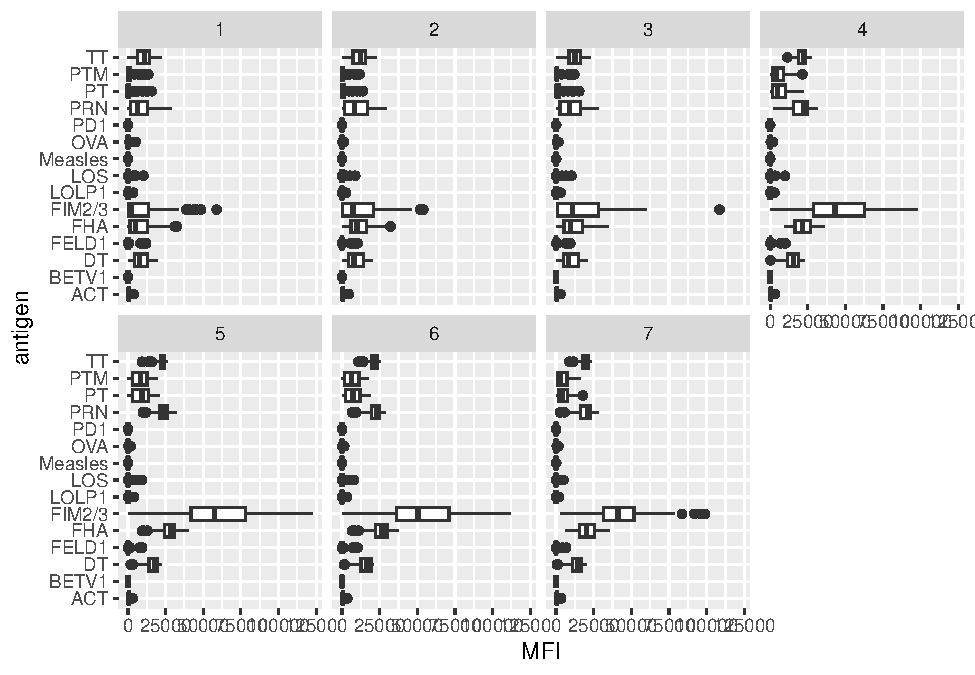
\includegraphics{lab-19-143_files/figure-latex/unnamed-chunk-24-1.pdf}
Q14. What antigens show differences in the level of IgG1 antibody titers
recognizing them over time? Why these and not others? FIM2/3 shows
change over multiple visits.

\begin{Shaded}
\begin{Highlighting}[]
\FunctionTok{ggplot}\NormalTok{(ig1) }\SpecialCharTok{+}
  \FunctionTok{aes}\NormalTok{(MFI, antigen, }\AttributeTok{col=}\NormalTok{infancy\_vac ) }\SpecialCharTok{+}
  \FunctionTok{geom\_boxplot}\NormalTok{(}\AttributeTok{show.legend =} \ConstantTok{FALSE}\NormalTok{) }\SpecialCharTok{+} 
  \FunctionTok{facet\_wrap}\NormalTok{(}\FunctionTok{vars}\NormalTok{(infancy\_vac, visit), }\AttributeTok{nrow=}\DecValTok{2}\NormalTok{)}
\end{Highlighting}
\end{Shaded}

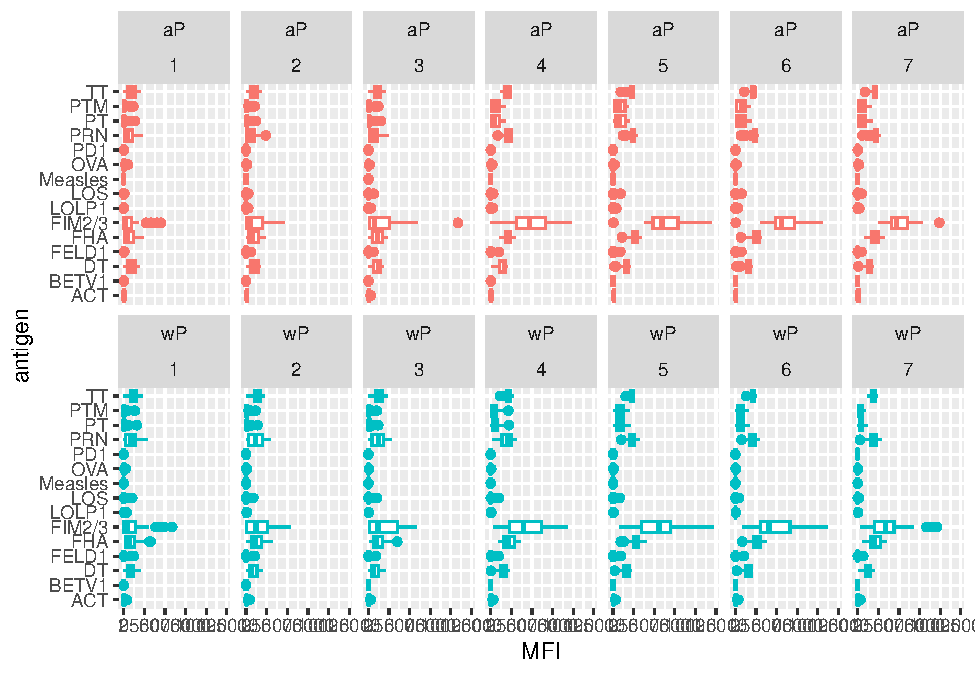
\includegraphics{lab-19-143_files/figure-latex/unnamed-chunk-25-1.pdf}

Q15. Filter to pull out only two specific antigens for analysis and
create a boxplot for each. You can chose any you like. Below I picked a
``control'' antigen (``Measles'', that is not in our vaccines) and a
clear antigen of interest (``FIM2/3'', extra-cellular fimbriae proteins
from B. pertussis that participate in substrate attachment).

\begin{Shaded}
\begin{Highlighting}[]
\FunctionTok{filter}\NormalTok{(ig1, antigen}\SpecialCharTok{==}\StringTok{"Measles"}\NormalTok{) }\SpecialCharTok{\%\textgreater{}\%}
  \FunctionTok{ggplot}\NormalTok{() }\SpecialCharTok{+}
  \FunctionTok{aes}\NormalTok{(MFI, }\AttributeTok{col=}\NormalTok{infancy\_vac) }\SpecialCharTok{+}
    \FunctionTok{geom\_boxplot}\NormalTok{(}\AttributeTok{show.legend =} \ConstantTok{FALSE}\NormalTok{) }\SpecialCharTok{+}
  \FunctionTok{facet\_wrap}\NormalTok{(}\FunctionTok{vars}\NormalTok{(visit)) }\SpecialCharTok{+}
  \FunctionTok{theme\_bw}\NormalTok{() }\SpecialCharTok{+}
  \FunctionTok{labs}\NormalTok{(}\AttributeTok{title =} \StringTok{"Measles Antigen per Visit (aP red, wP teal)"}\NormalTok{)}
\end{Highlighting}
\end{Shaded}

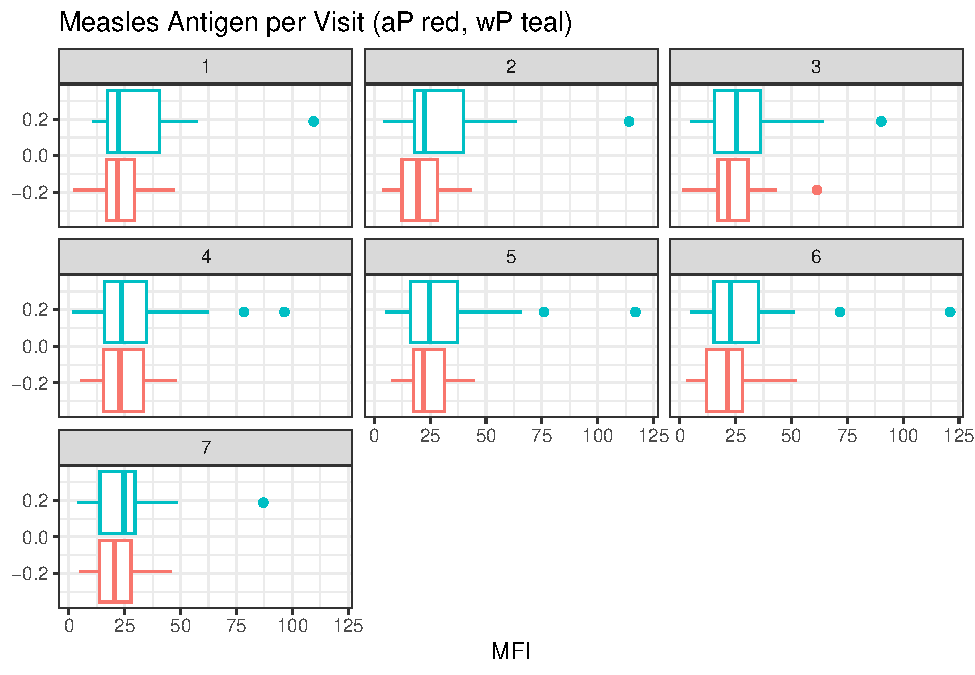
\includegraphics{lab-19-143_files/figure-latex/unnamed-chunk-26-1.pdf}

\begin{Shaded}
\begin{Highlighting}[]
\FunctionTok{filter}\NormalTok{(ig1, antigen}\SpecialCharTok{==}\StringTok{"FIM2/3"}\NormalTok{) }\SpecialCharTok{\%\textgreater{}\%}
  \FunctionTok{ggplot}\NormalTok{() }\SpecialCharTok{+}
  \FunctionTok{aes}\NormalTok{(MFI, }\AttributeTok{col=}\NormalTok{infancy\_vac) }\SpecialCharTok{+}
    \FunctionTok{geom\_boxplot}\NormalTok{(}\AttributeTok{show.legend =} \ConstantTok{FALSE}\NormalTok{) }\SpecialCharTok{+}
  \FunctionTok{facet\_wrap}\NormalTok{(}\FunctionTok{vars}\NormalTok{(visit)) }\SpecialCharTok{+}
  \FunctionTok{theme\_bw}\NormalTok{() }\SpecialCharTok{+}
  \FunctionTok{labs}\NormalTok{(}\AttributeTok{title =} \StringTok{"FIM2/3 Antigen per Visit (aP red, wP teal)"}\NormalTok{)}
\end{Highlighting}
\end{Shaded}

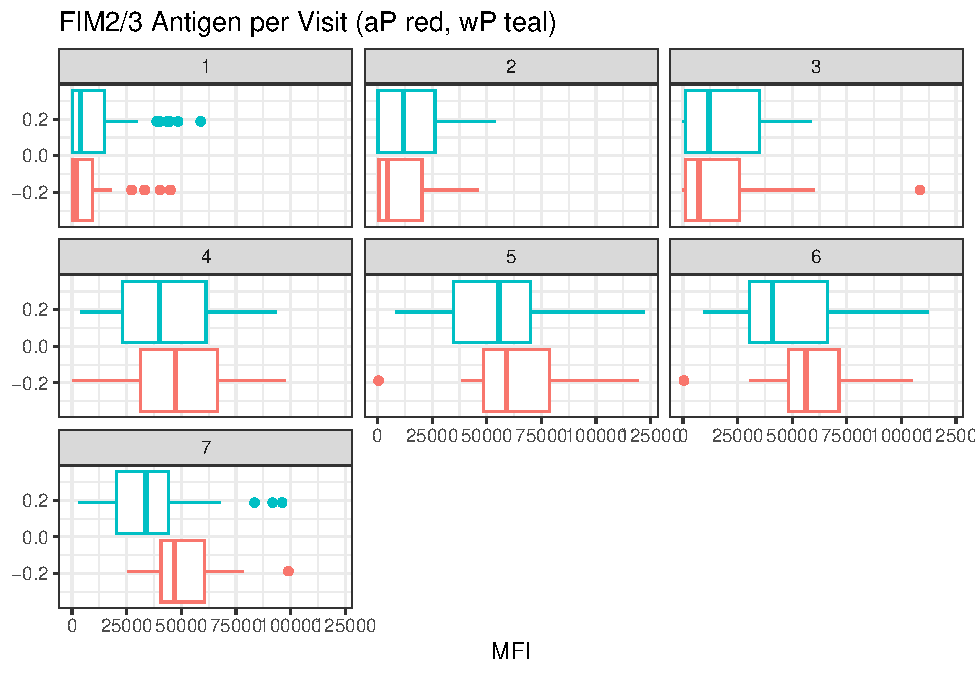
\includegraphics{lab-19-143_files/figure-latex/unnamed-chunk-27-1.pdf}

\begin{enumerate}
\def\labelenumi{\arabic{enumi}.}
\setcounter{enumi}{15}
\tightlist
\item
  What do you notice about these two antigens time course and the FIM2/3
  data in particular? Over time, measles antigen stays relatively low.
  FIM2/3 increases per visit.
\end{enumerate}

Q17. Do you see any clear difference in aP vs.~wP responses? At least in
FIM2/3, aP vaccines show higher antigen response through multiple
visits. However in the measles data, the aP and wP show similar
responses.

\hypertarget{obtaining-cmi-pb-rnaseq-data}{%
\section{Obtaining CMI-PB RNASeq
Data}\label{obtaining-cmi-pb-rnaseq-data}}

\begin{Shaded}
\begin{Highlighting}[]
\CommentTok{\# Read in file}
\NormalTok{url }\OtherTok{\textless{}{-}} \StringTok{"https://www.cmi{-}pb.org/api/v2/rnaseq?versioned\_ensembl\_gene\_id=eq.ENSG00000211896.7"}
\NormalTok{rna }\OtherTok{\textless{}{-}} \FunctionTok{read\_json}\NormalTok{(url, }\AttributeTok{simplifyVector =} \ConstantTok{TRUE}\NormalTok{)}

\CommentTok{\#meta \textless{}{-} inner\_join(specimen, subject)}
\NormalTok{ssrna }\OtherTok{\textless{}{-}} \FunctionTok{inner\_join}\NormalTok{(rna, meta)}
\end{Highlighting}
\end{Shaded}

\begin{verbatim}
## Joining with `by = join_by(specimen_id)`
\end{verbatim}

Q18. Make a plot of the time course of gene expression for IGHG1 gene
(i.e.~a plot of visit vs.~tpm).

\begin{Shaded}
\begin{Highlighting}[]
\FunctionTok{ggplot}\NormalTok{(ssrna) }\SpecialCharTok{+}
  \FunctionTok{aes}\NormalTok{(visit, tpm, }\AttributeTok{group=}\NormalTok{subject\_id) }\SpecialCharTok{+}
  \FunctionTok{geom\_point}\NormalTok{() }\SpecialCharTok{+}
  \FunctionTok{geom\_line}\NormalTok{(}\AttributeTok{alpha=}\FloatTok{0.2}\NormalTok{)}
\end{Highlighting}
\end{Shaded}

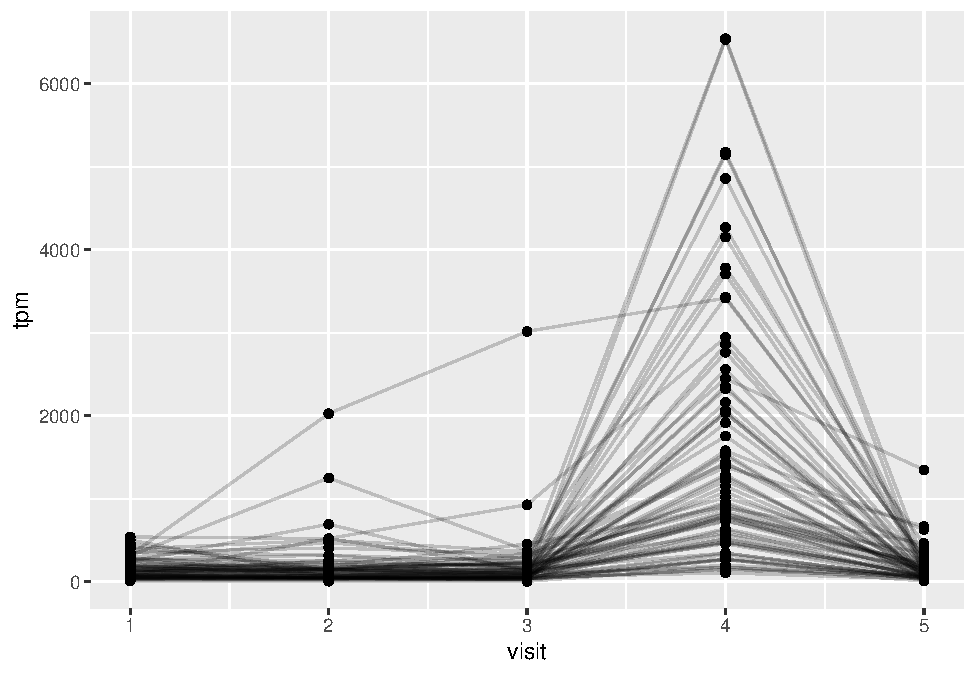
\includegraphics{lab-19-143_files/figure-latex/unnamed-chunk-29-1.pdf}

Q19.: What do you notice about the expression of this gene (i.e.~when is
it at it's maximum level)? Maxes out at visit 4

Q20. Does this pattern in time match the trend of antibody titer data?
If not, why not? Nope. It doesn't waver/decrease afterwards.

\begin{Shaded}
\begin{Highlighting}[]
\FunctionTok{ggplot}\NormalTok{(ssrna) }\SpecialCharTok{+}
  \FunctionTok{aes}\NormalTok{(tpm, }\AttributeTok{col=}\NormalTok{infancy\_vac) }\SpecialCharTok{+}
  \FunctionTok{geom\_boxplot}\NormalTok{() }\SpecialCharTok{+}
  \FunctionTok{facet\_wrap}\NormalTok{(}\FunctionTok{vars}\NormalTok{(visit))}
\end{Highlighting}
\end{Shaded}

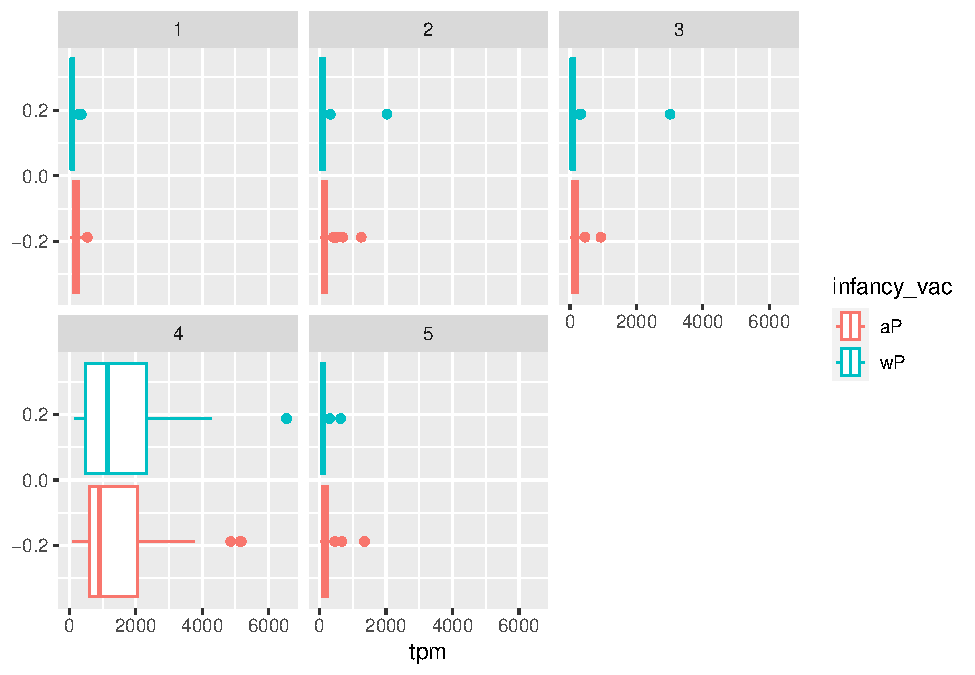
\includegraphics{lab-19-143_files/figure-latex/unnamed-chunk-30-1.pdf}

\begin{Shaded}
\begin{Highlighting}[]
\NormalTok{ssrna }\SpecialCharTok{\%\textgreater{}\%}  
  \FunctionTok{filter}\NormalTok{(visit}\SpecialCharTok{==}\DecValTok{4}\NormalTok{) }\SpecialCharTok{\%\textgreater{}\%} 
  \FunctionTok{ggplot}\NormalTok{() }\SpecialCharTok{+}
    \FunctionTok{aes}\NormalTok{(tpm, }\AttributeTok{col=}\NormalTok{infancy\_vac) }\SpecialCharTok{+} \FunctionTok{geom\_density}\NormalTok{() }\SpecialCharTok{+} 
    \FunctionTok{geom\_rug}\NormalTok{() }
\end{Highlighting}
\end{Shaded}

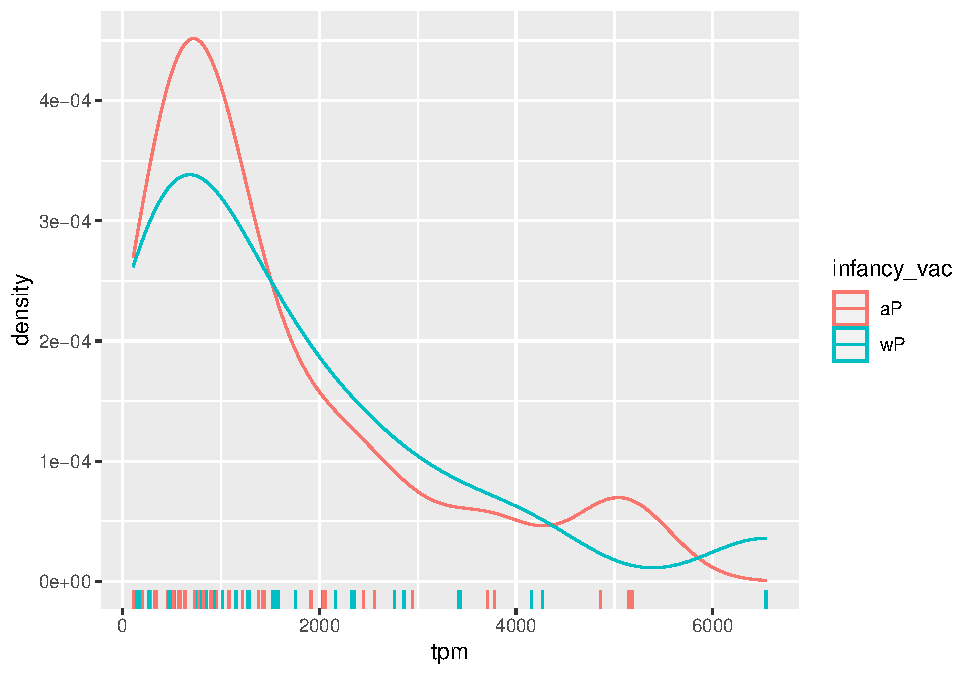
\includegraphics{lab-19-143_files/figure-latex/unnamed-chunk-31-1.pdf}

\end{document}
